%%%%%%%%%%%%%%%%%%%%%%%%%%%%%%%%%%%%%%%%%
% Dreuw & Deselaer's Poster
% LaTeX Template
% Version 1.0 (11/04/13)
%
% Created by:
% Philippe Dreuw and Thomas Deselaers
% http://www-i6.informatik.rwth-aachen.de/~dreuw/latexbeamerposter.php
%
% This template has been downloaded from:
% http://www.LaTeXTemplates.com
%
% License:
% CC BY-NC-SA 3.0 (http://creativecommons.org/licenses/by-nc-sa/3.0/)
%
%%%%%%%%%%%%%%%%%%%%%%%%%%%%%%%%%%%%%%%%%

%----------------------------------------------------------------------------------------
%	PACKAGES AND OTHER DOCUMENT CONFIGURATIONS
%----------------------------------------------------------------------------------------

\documentclass[final,hyperref={pdfpagelabels=false}]{beamer}

\usepackage[orientation=portrait,size=a0,scale=1.4]{beamerposter} % Use the beamerposter package for laying out the poster with a portrait orientation and an a0 paper size

\usetheme{I6pd2} % Use the I6pd2 theme supplied with this template

\usepackage[english]{babel} % English language/hyphenation

\usepackage{amsmath,amsthm,amssymb,latexsym} % For including math equations, theorems, symbols, etc

%\usepackage{times}\usefonttheme{professionalfonts}  % Uncomment to use Times as the main font
%\usefonttheme[onlymath]{serif} % Uncomment to use a Serif font within math environments

\boldmath % Use bold for everything within the math environment

\usepackage{booktabs} % Top and bottom rules for tables

\graphicspath{{figures/}} % Location of the graphics files

\usecaptiontemplate{\small\structure{\insertcaptionname~\insertcaptionnumber: }\insertcaption} % A fix for figure numbering

%----------------------------------------------------------------------------------------
%	TITLE SECTION 
%----------------------------------------------------------------------------------------

\title{\huge Photon pair-production Resolution Studies of the High Granularity Calorimeter of the CMS experiment at the LHC at CERN} % Poster title

\author{Stephan Koenigstorfer, Johannes Prosser} % Author(s)

\institute{Imperial College London, High Energy Physics Group} % Institution(s)

%----------------------------------------------------------------------------------------
%	FOOTER TEXT
%----------------------------------------------------------------------------------------

\newcommand{\leftfoot}{http://www.LaTeXTemplates.com} % Left footer text

\newcommand{\rightfoot}{john@smith.com} % Right footer text

%----------------------------------------------------------------------------------------

\begin{document}

\addtobeamertemplate{block end}{}{\vspace*{2ex}} % White space under blocks

\begin{frame}[t] % The whole poster is enclosed in one beamer frame

\begin{columns}[t] % The whole poster consists of two major columns, each of which can be subdivided further with another \begin{columns} block - the [t] argument aligns each column's content to the top

\begin{column}{.02\textwidth}\end{column} % Empty spacer column

\begin{column}{.465\textwidth} % The first column

%----------------------------------------------------------------------------------------
%	OBJECTIVES
%----------------------------------------------------------------------------------------

\begin{block}{Introduction}

		The Large Hadron Collider (LHC) is currently in the middle of the second Long Shutdown, which is used as part of a larger program to upgrade the collider to the High Luminosity LHC by the mid 2020s. The main goal of coming upgrades to the LHC is to increase the instantaneous luminosities which the collider can produce, in order to zero in on anomalies in the data. Figure \ref*{timeline} shows the past and expected future luminosities achieved. The big jump in instantaneous luminosity during the Third Long Shutdown (LS3), is the switch to the High Luminosity LHC (HL-LHC). 
		\begin{column}{0.6\textwidth}
		\begin{figure}
			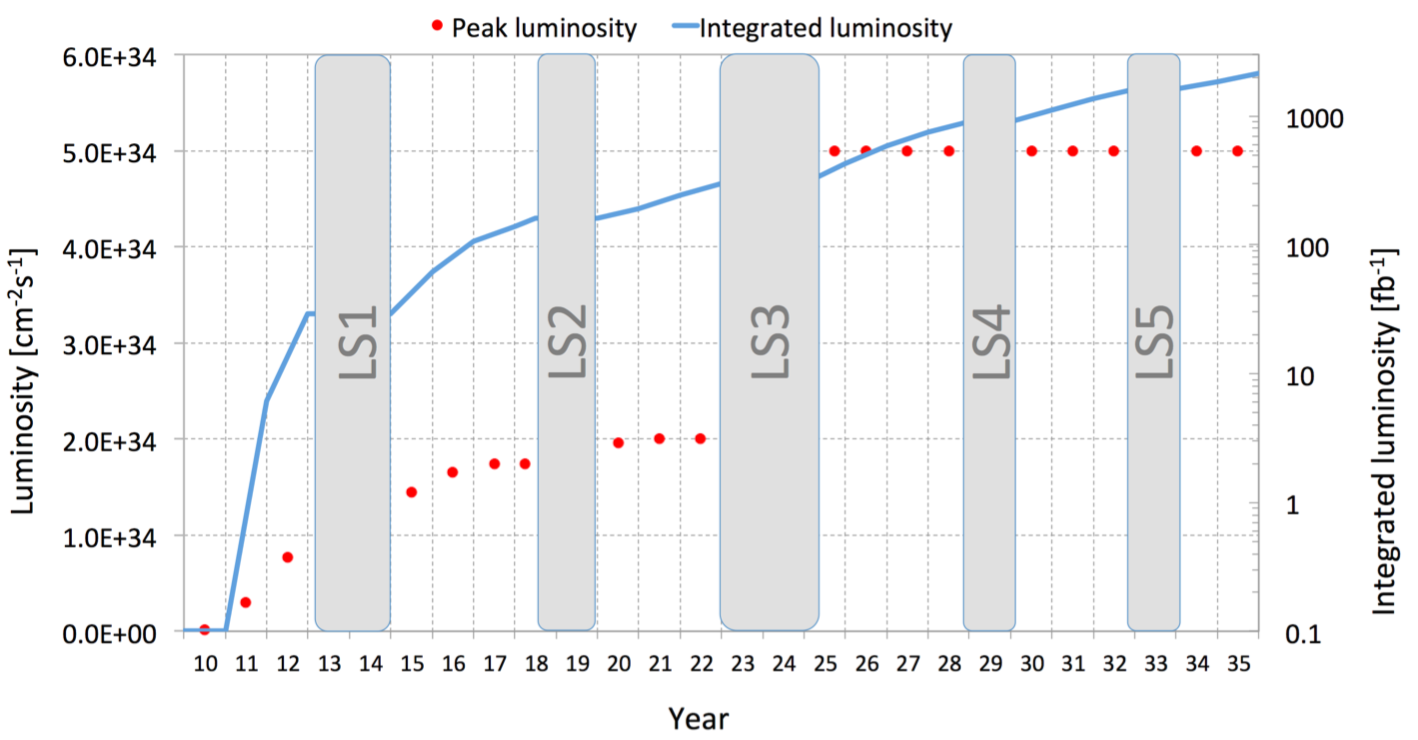
\includegraphics[width=\linewidth]{LHC_upgrade_timeplan.png}
				\caption{Instantaneous luminosity (red dots) and Integrated luminosity (blue line) of the LHC, during various phases in the upgrade cycle.}
			\label{timeline}
		\end{figure}
		\end{column}
		\begin{column}{0.01\textwidth}\end{column}
		\begin{column}{0.29\textwidth}
				\\As part of the H-LHC upgrade, the dectector systems on the experiments are also being upgraded. This project is specifically concerned with the High Granularity Calorimeter (HGCAL) of the CMS
		\end{column}

		experiment, and studying how the new detector will respond to photons with different detector settings. The detector will produce data at rates exceeding 100TB/s, which far exceeds the capacity of the read out channels. Therefore, a decision whether or not to read out the data (trigger decision) has to be made on detector within a small latency. The studies in presented in this poster aim to inform the development of such a trigger algorithm.

\end{block}

%----------------------------------------------------------------------------------------
%	Background
%----------------------------------------------------------------------------------------
            
\begin{block}{Background: The CMS HGCAL}

	The CMS HGCAL is radially symmetric every 60$^\circ$ around the beam axis. Longitudinally, it is made up of 52 layers, most of which use hexagonal Silicone Wafers as the detector material. On the Silicon wafers there are hexagonal subdivisions of area either 

\end{block}

\begin{block}{Background: Pileup}



	There is pileup. Basically there are always some particles flying around as a background. These also get caught in the detector, but have nothing to do with the event being observed. This is called pileup.

	The HGCAL is mainly made out of xx layers of small hexagonal silican wafers, in which particles deposit their energy. This energy is then read out via an HGC read out chip (HGROC) and passed to a motherboard. 3 HGCROCs run into one motherboard. There are also some layers of scinitllator material in the hadronic calorimeter. 

	The detector geometry is usually destribed in reduced coordinates and in eta and phi. Eta is some complicated shit. 
\end{block}


%----------------------------------------------------------------------------------------
%	Methods
%----------------------------------------------------------------------------------------

\begin{block}{Methods}
	We are working on data compiled from CMSSW, the advanced software produced by the CMS team to simulate the physics of incoming collisions. These are very computationally heavy, so we work on the output files of these simulations. These files are root ntuples, containing segmented data of all the results. We then simulate a detector environment and different trigger mechanisms, and analyse the resulting output. 

	There are several clustering mechanisms:
	\begin{enumerate}
		\item Triggering on the generated particle (only in theory).
		\item Triggering on all trigger cells above a threshold.
		\item Triggering on trigger cells whose energy content is significantly higher than the surroundings.
		\item Triggering on groups of trigger cells whose energy content is significantly higher than the surroundings.
	\end{enumerate}
	
	\\
	Hi Tina \\
	

\end{block}

%----------------------------------------------------------------------------------------
%	METHODS
%----------------------------------------------------------------------------------------

\begin{block}{Methods}

\begin{itemize}
\item Maecenas Vel Nisl Elit
\begin{itemize}
\item Suspendisse potenti. Fusce a est eget turpis rhoncus varius sed sed dui. Cras justo nibh, bibendum a cursus eget, consequat et dui. Maecenas vel nisl elit, sed dignissim dolor. 
\item In hac habitasse platea dictumst.
\end{itemize}

\item Viewpoint Matching Constraints
\begin{itemize}
\item Cum sociis natoque penatibus et magnis dis parturient montes, nascetur ridiculus mus. 
\item Proin in nisi diam.
\item Nam ultricies pellentesque nunc, ultrices volutpat nisl ultrices a.
\end{itemize}

\item Volutpat 
\begin{itemize}
\item Duis semper lorem eget dui dignissim porttitor.
\item Nulla facilisi. In ullamcorper lorem quis dolor.
\end{itemize}
\end{itemize}

\end{block}

%----------------------------------------------------------------------------------------
%	MATHEMATICAL SECTION
%----------------------------------------------------------------------------------------

\begin{block}{Mathematical Section}

\begin{itemize}
\item Maecenas Ultricies Feugiat Velit Non Mattis.
\begin{itemize}
\item Duis ante erat, bibendum nec tempus nec, interdum quis est. Nulla at mollis tortor. Phasellus quis leo dolor, aliquam laoreet orci $X$ Donec dapibus sagittis neque eu nec, interdum quis est. $Y_n, n=1,\cdots,N$ ndum nec tempus nec, interd
\begin{align*}
X \rightarrow r(X) & = \arg \max_{c} \Big\{ \max_n \big\{ \sum_{x_i \in X} \delta(x_i,Y_{n,c})\big\} \Big\} 
\end{align*}
\item Cras faucibus scelerisque cursus. Proin ut vestibulum augue. $\delta(x_i,Y_{n,c})$
\end{itemize}
\item Fusce tempus arcu id ligula varius dictum. Donec ut nisl dui, ac consectetur elit. In nec enim porta augue venenatis sollicitudin. Phasellus quis nunc neque. Suspendisse mauris diam, suscipit non gravida in, placerat id enim. Ut nec ipsum in lectus ultrices sagittis.
\end{itemize}

\end{block}

%----------------------------------------------------------------------------------------

\end{column} % End of the first column

\begin{column}{.03\textwidth}\end{column} % Empty spacer column
 
\begin{column}{.465\textwidth} % The second column

%----------------------------------------------------------------------------------------
%	RESULTS
%----------------------------------------------------------------------------------------

\begin{block}{Results}

	

	\begin{figure}
		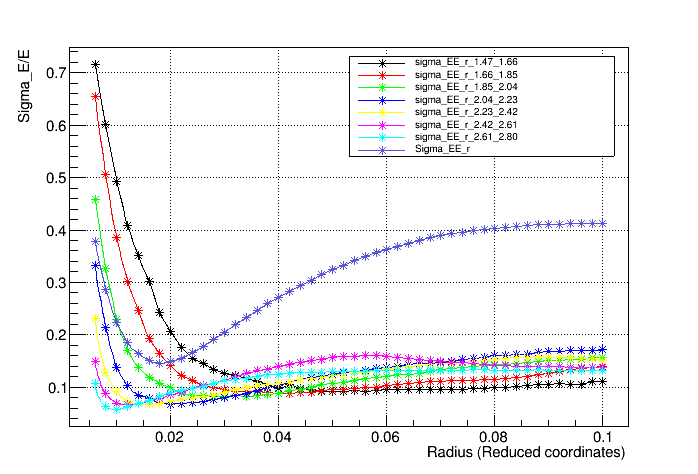
\includegraphics[width=0.4\linewidth]{SigmaEvsR.png}
		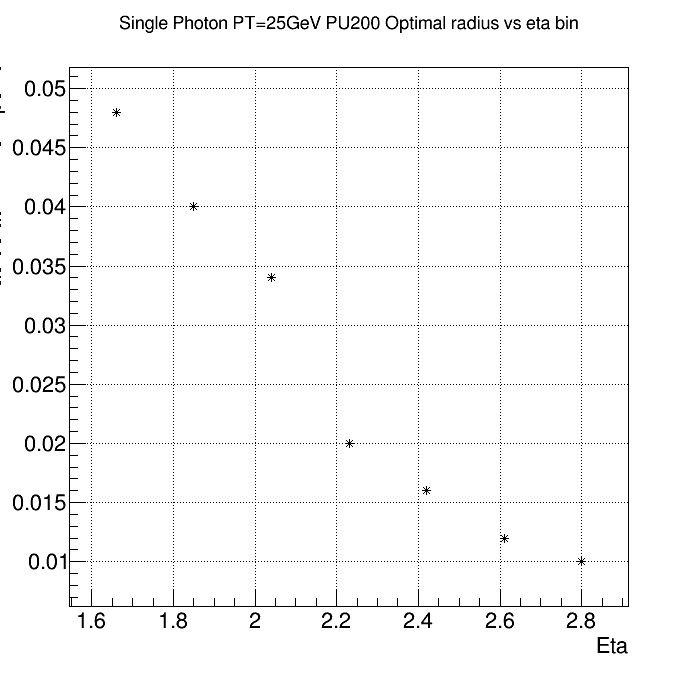
\includegraphics[width=0.4\linewidth]{SingleGammaPT25GeVPU200OptimalRadiusbyEta.png}
			\caption{This shows the standardized error on the energy measurement (y-axis) plotted against different radii for the whole detector (dark blue line), and for individual eta segments(other lines). The key result is that the smallest achievable error significantly decreases when different radii are used for different eta segments.}
	\end{figure}

	
     
\end{block}



%----------------------------------------------------------------------------------------
%	CONCLUSION
%----------------------------------------------------------------------------------------

\begin{block}{Conclusion}

\begin{itemize}
\item Opet volutpat ligula. Duis semper lorem eget dui dignissim porttitor. Nulla facilisi. In ullamcorper lorem quis dolor iaculis nec egestas enim ultricies. Cras ut mauris elit, ut lacinia dui. Proin in ante et libero hendrerit iacunlis.
\item Nulla eu erat a urna laoreet auctor id a turpis. Nam mollis tristique neque eu luctus. Suspendisse rutrum congue nisi sed convallis. 
\item Aenean id neque dolor.
\item Opet volutpat ligula. Duis semper lorem eget dui dignissim porttitor. Nulla facilisi. In ullamcorper lorem quis dolor iaculis nec egestas enim ultricies. Cras ut mauris elit, ut lacinia dui. Proin in ante et libero hendrerit iaculis.
\end{itemize}

\end{block}

%----------------------------------------------------------------------------------------
%	REFERENCES
%----------------------------------------------------------------------------------------

\begin{block}{References}
        
\nocite{*} % Insert publications even if they are not cited in the poster
\small{\bibliographystyle{unsrt}
\bibliography{sample}}

\end{block}

%----------------------------------------------------------------------------------------
%	ACKNOWLEDGEMENTS
%----------------------------------------------------------------------------------------

\begin{block}{Acknowledgments}

\begin{itemize}
\item Nam mollis tristique neque eu luctus. Suspendisse rutrum congue nisi sed convallis. Aenean id neque dolor. Pellentesque habitant morbi tristique senectus et netus et malesuada fames ac turpis egestas.
\end{itemize}

\end{block}

%----------------------------------------------------------------------------------------
%	CONTACT INFORMATION
%----------------------------------------------------------------------------------------

\setbeamercolor{block title}{fg=black,bg=orange!70} % Change the block title color

\begin{block}{Contact Information}

\begin{itemize}
\item Web: \href{http://www.university.edu/smithlab}{http://www.university.edu/smithlab}
\item Email: \href{mailto:john@smith.com}{john@smith.com}
\item Phone: +1 (000) 111 1111
\end{itemize}

\end{block}

%----------------------------------------------------------------------------------------

\end{column} % End of the second column

\begin{column}{.015\textwidth}\end{column} % Empty spacer column

\end{columns} % End of all the columns in the poster

\end{frame} % End of the enclosing frame

\end{document}
